%! TEX program = xelatex

\documentclass{article}
\usepackage[a4paper, margin=3cm]{geometry}
\setlength{\parindent}{0pt}
\setlength{\parskip}{1em}
\usepackage{fontspec}
\setmainfont{Lato}

\usepackage{amsmath,amssymb,amsthm}
%\usepackage{hyperref}
\usepackage{verbatim}
\usepackage{graphicx}
%\usepackage{pgfplots}
%\pgfplotsset{compat=1.16}

\title{TIEA381 Demo 1}
\author{Mikael Myyrä}
\date{\number\day.\number\month.\number\year}

\begin{document}

\maketitle

\section*{1.}

Matlab-koodi:

\verbatiminput{w1_1.m}

tulostaa

\verbatiminput{|"octave w1_1.m"}

Epästabiilissa versiossa double- ja single-tarkkuuksien väliset erot ovat
huomattavat, kun taas stabii\-lissa ei eroa ole tällä näyttötarkkuudella lainkaan.


\section*{2.}

Matlab-koodi:

\verbatiminput{w1_2.m}

tulostaa

\verbatiminput{|"octave w1_2.m"}


\section*{3.}

Etsitään lukua $x$, jolle $x^3 = 1002 \iff x^3 - 1002 = 0$.
Merkitään $f(x) = x^3 - 1002$, jolloin $f'(x) = 3x^2$.
Etsitään nollakohta Newtonin menetelmällä.

Matlab-koodi:

\verbatiminput{w1_3.m}

tulostaa

\verbatiminput{|"octave w1_3.m"}

\section*{4-5.}

Ympyrän segmentin ala on
\[
  a = \frac{R^2}{2}(\varphi - \sin \varphi).
\]
Sijoittamalla tunnetut arvot $a = 0.1 (m^2)$ ja $R = 1 (m)$ saadaan
\begin{align*}
  0.1 &= \frac{1}{2}(\varphi - \sin \varphi) \\
  \varphi - \sin \varphi - 0.2 &= 0.
\end{align*}
Ratkaisun Matlab-koodi:

\verbatiminput{w1_4.m}

Tulostaa

\verbatiminput{|"octave w1_4.m"}

\section*{6-7.}

\[
  \frac{1}{\sqrt{f}} = -2\log_{10} \Big(\frac{2.51}{\text{Re} \cdot \sqrt{f}}\Big)
\]
Muuttujanvaihto $x = \frac{1}{\sqrt{f}}$ (jolloin $f = \frac{1}{x^2}$):
\[
  x = -2\log_{10} \Big(\frac{2.51x}{\text{Re}}\Big)
\]
Kiintopistemenetelmään sopiva muoto:
\[
  x - \Big(-2\log_{10} \Big(\frac{2.51x}{\text{Re}}\Big)\Big) = 0
\]

Matlab-koodi:

\verbatiminput{w1_6.m}

piirtää

\begin{center}
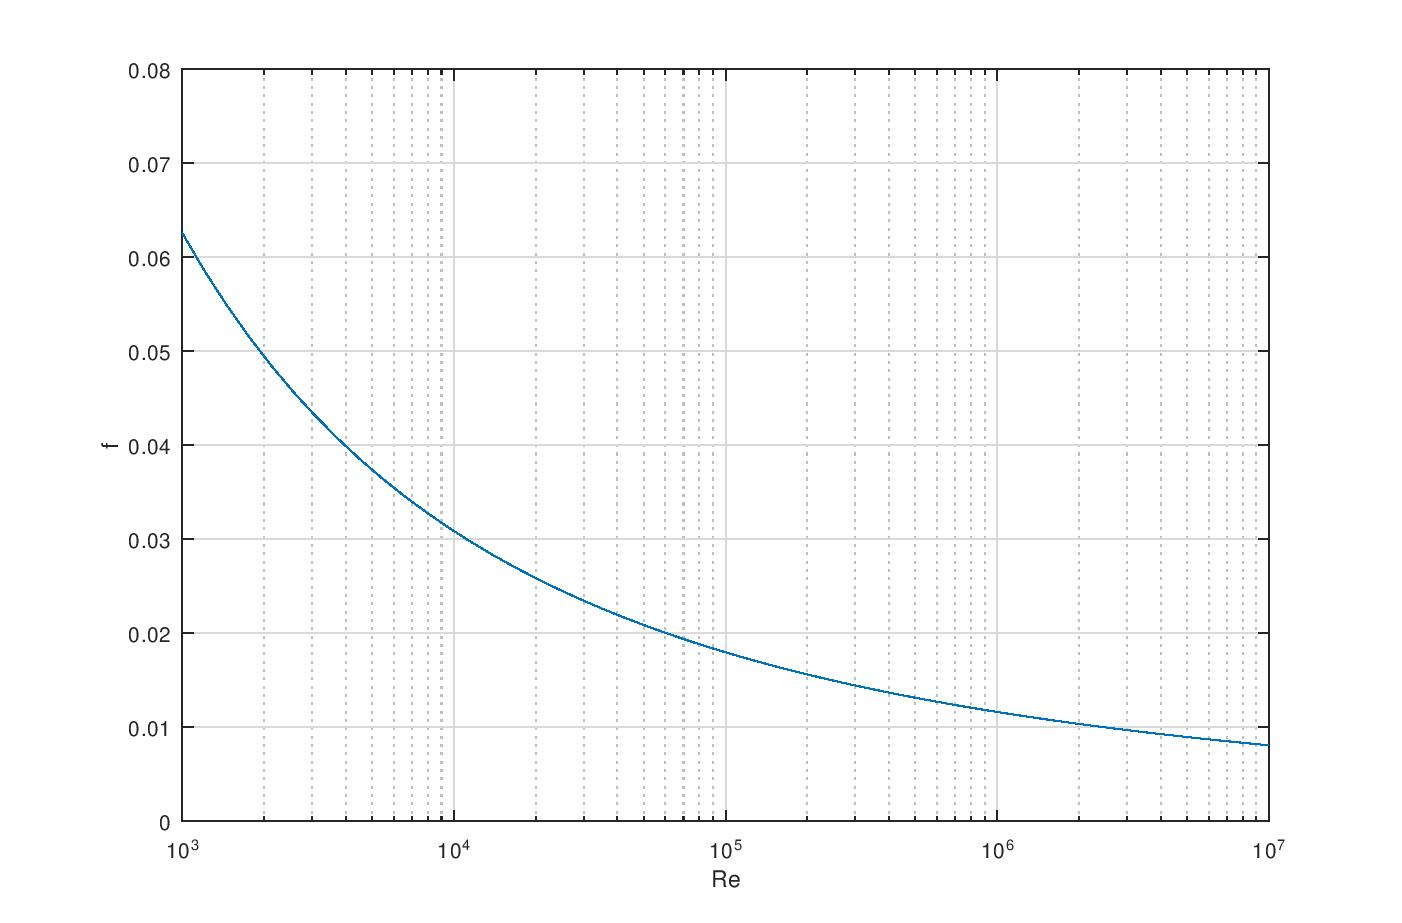
\includegraphics[width=350pt]{w1_6.jpg}
\end{center}

\end{document}
